\section{Result Analysis}
\label{sec:trajectory}
In this section, we perform analysis of archetypes identified by our model. We first describe the discovered archetypes of all researchers in~\Cref{sec:acad}. Then, we examine gender variation in academic trajectory in~\Cref{sec:discussion} and effect of archetype and gender on grant income in~\Cref{sec:grant}. Finally, we describe discovered archetypes for the largest Stack Exchange community, StackOverflow in~\Cref{sec:stack}.

\subsection{Discovered Archetypes of Academics}
\label{sec:acad}
Our analysis reveals four dominant archetypes: \emph{Steady}, \emph{Diverse}, \emph{Evolving} and \emph{Diffuse}. We chose the number of clusters $C=4$ using the elbow method \cite{elbow:2001}: data log-likelihoods increased rapidly till four clusters with much slower increase beyond that. Further, we chose the number of states per cluster, $K=5$: beyond five states, KL divergence\cite{kl:1951} between mean vectors of new states with previous states started reducing rapidly, indicating redundant states.

We also conducted t-test to validate differences among the identified archetypes. Specifically, paired-sample t-test \cite{goulden:1949} is conducted between likelihood values of data points assigned to an archetype with their likelihood values obtained from rest of the archetypes. For instance, for each archetype pair $(p, q)$, we conduct paired t-test between $\log P(X_i| \lambda^p)$ and $\log P(X_i| \lambda^q)$ $\forall i \ni c_i=p$. Note that test results for archetype pair $(p, q)$ are not symmetric.
We observed that all archetype pairs are significantly different ($p < .001$) from each other. Now, we proceed to discuss what is common to these discovered archetypes before examining each one in detail.

\begin{figure*}[tbh]
	\centering
	\begin{subfigure}{\textwidth}
		\centering
		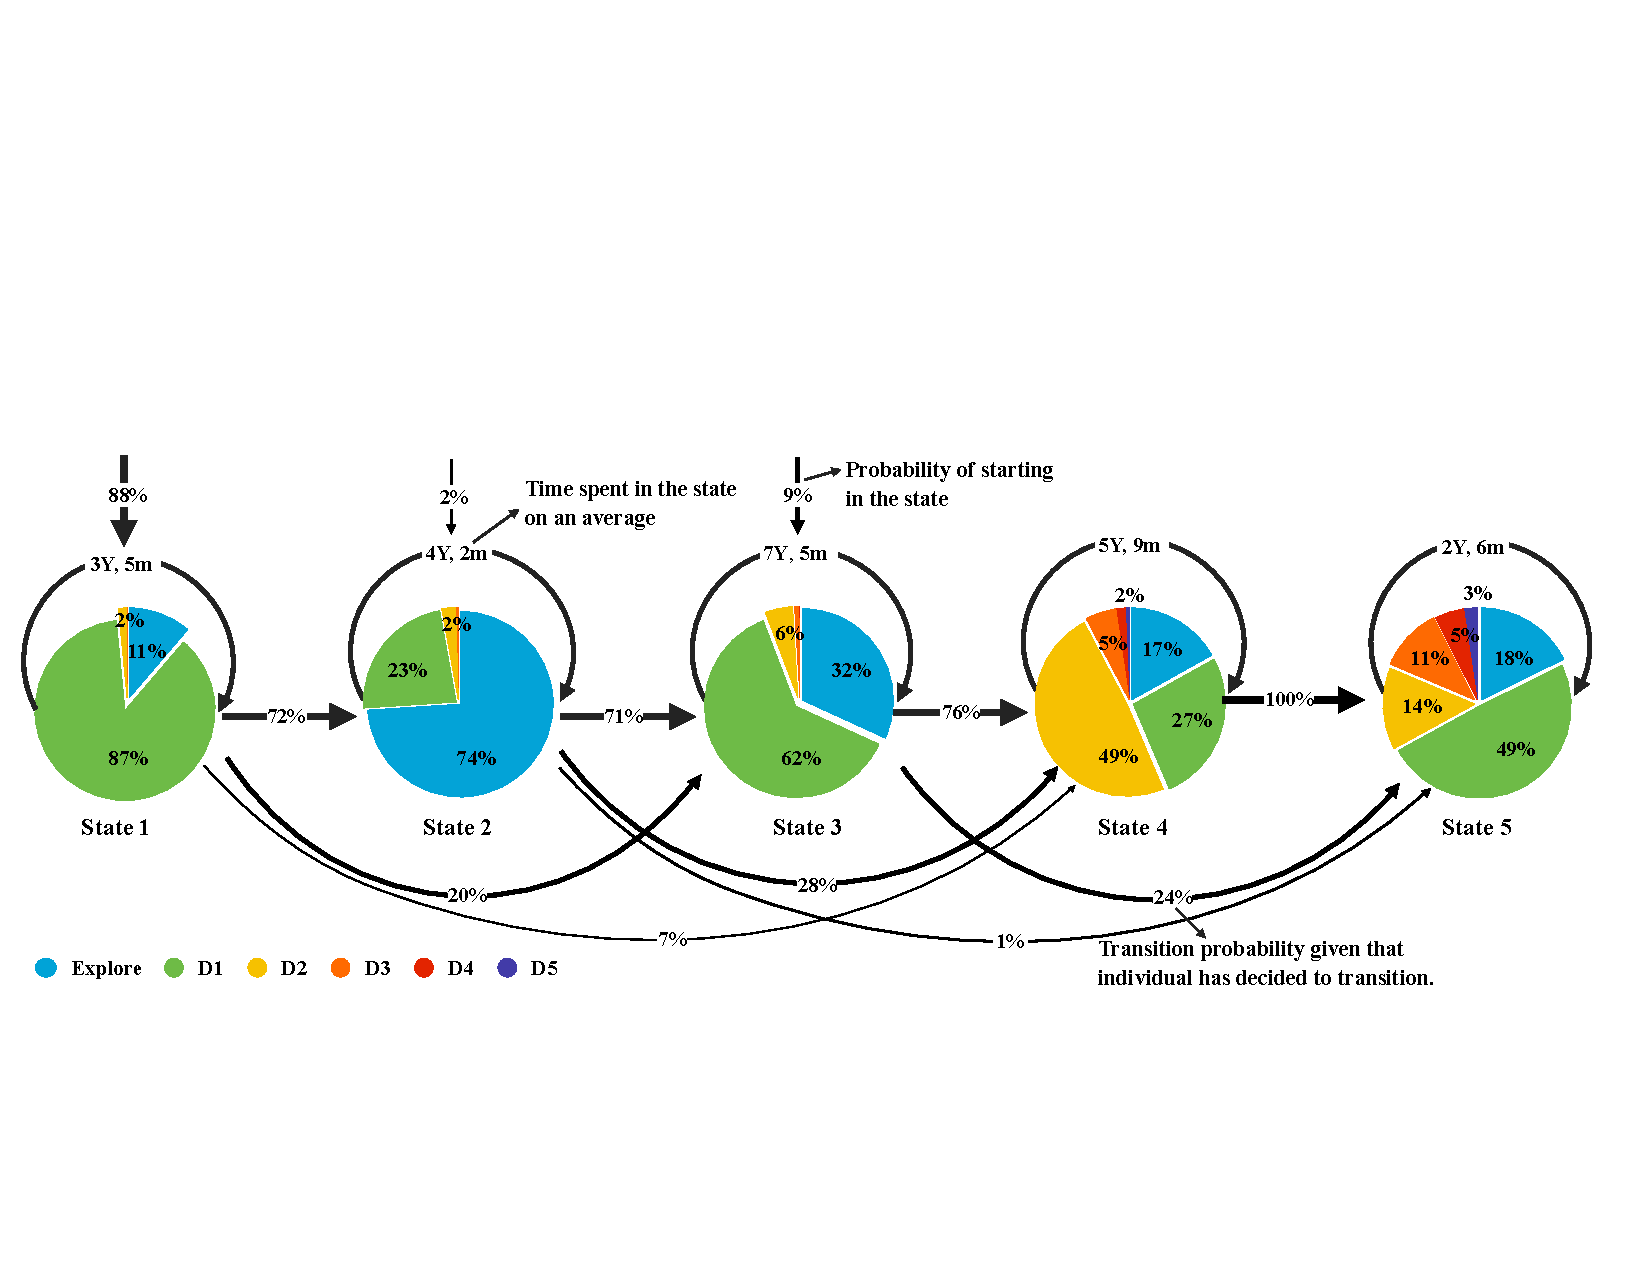
\includegraphics[width=1\linewidth,height=6.4cm]{figures/Cluster4_Self.pdf}
	\end{subfigure}
	\caption{%\small
	\label{fig:acadclusters} Trajectory (state sequence) for \emph{Steady} archetype in the Academic Dataset. Each pie is a \emph{latent state} or \emph{behavioral stage} in the trajectory. It denotes the mean proportion of papers published in each \emph{Area of Interest}'s in the latent state. Each state is also labeled with the average amount of time spent in the state. For example, in this cluster, 87\% of publications in the first 3.5 years are in the author's primary \texttt{AoI} $D_1$ while rest 11\% are in exploring other areas. The arrows on the top of each pie show the prior probability for starting in that state. As we learn a left-to-right G-HMM, an author can transition to its immediate next state or any later latent states. Each transition is labeled with the corresponding conditional transition probability i.e., transition probability given that the user has decided to transition. The arrows thickness is proportional to its weight. Authors in this cluster exhibit \emph{steady} research interest in their primary \texttt{AoI} $D_1$. Some authors start contributing dominantly in their secondary \texttt{AoI}, $D_2$ in State 4. Though, they return to spending around half of their effort in $D_1$ in State 5.
	}
	\label{fig:academic}
\end{figure*}

\begin{table}[!h]
	\centering
	\begin{tabular}{p{40mm} p{25mm} p{25mm} p{25mm} p{25mm}@{}}
		\toprule
		{Behavioral Stage}  & {Steady} & {Diverse} & {Evolving} & {Diffuse} \\
		\midrule
		Stage \textbf{1}& \{3Y, 5m\} \newline $\mathbf{D_1}$ (87\%) \newline Ex (11\%) &
		\{3Y, 3m\} \newline $\mathbf{D_1}$ (88\%)\newline Ex (11\%)&
		\{2Y, 9m\} \newline $\mathbf{D_1}$ (72\%)\newline Ex (24\%) &
		\{2Y, 7m\} \newline $\mathbf{D_1}$(76\%) \newline Ex (22\%) \\\\
		Stage \textbf{2} &  \{4Y, 2m\} \newline \textbf{Ex} (74\%)\newline ${D_1}$ (23\%) &
		\{2Y, 6m \} \newline \textbf{Ex} (80\%)\newline ${D_1}$ (16\%) &
		\{2Y, 9m \} \newline \textbf{Ex} (83\%)\newline ${D_1}$ (12\%) &
		\{3Y, 7m \} \newline \textbf{Ex} (91\%) \\\\
		Stage \textbf{3} & \{7Y, 5m\} \newline $\mathbf{D_1}$ (62\%) \newline \textbf{Ex} (32\%)  &
		\{5Y, 6m\} \newline $\mathbf{D_1}$ (73\%) \newline Ex (17\%) &
		\{6Y, 2m\} \newline $\mathbf{D_1}$ (33\%) \newline \textbf{Ex} (28\%) \newline $\mathbf{D_2}$ (24\%)&
		\{8Y, 5m\} \newline $\mathbf{D_1}$ (50\%) \newline \textbf{Ex} (39\%) \\\\
		Stage \textbf{4} & \{5Y, 9m\} \newline $\mathbf{D_2}$ (49\%) \newline $\mathbf{D_1}$ (27\%) \newline Ex (17\%) &
		\{5Y, 6m\} \newline $\mathbf{Ex}$ (46\%) \newline ${D_2}$ (20\%) \newline ${D_1}$ (17\%)&
		\{5Y\} \newline $\mathbf{D_2}$ (66\%) \newline $Ex$ (18\%)  &
		\{3Y, 9m\} \newline $\mathbf{D_2}$ (43\%) \newline $\mathbf{Ex}$ (26\%) \\\\
		Stage \textbf{5} & \{2Y, 6m\} \newline $\mathbf{D_1}$ (49\%) \newline {Ex} (18\%) \newline ${D_2}$ (14\%) &
		\{6Y, 3m\} \newline $\mathbf{D_4}$ (29\%) \newline \textbf{Ex} (20\%) \newline ${D_3}$ (14\%) \newline ${D_1}$ (14\%) &
		\{6Y, 5m\} \newline $\mathbf{D_3}$ (43\%) \newline {Ex} (19\%) \newline ${D_2}$ (14\%) &
		\{4Y, 1m\} \newline \textbf{Ex} (74\%) \\
		\bottomrule
	\end{tabular}
	\caption{
	\label{tab:mean} Learned mean vector for each latent state of four archetypes in the Academic Dataset. We list the \emph{Area-of-Interests} (\texttt{AoI}) in sorted order and annotate them with their \% contribution in the state. We only list significant \texttt{AoI} ($>$ 11\%) for each state. Each state is also labeled with its average duration in \{Years (Y), months (m)\}. The labels given to these clusters reflect our interpretation of the user behavior and make disambiguation of the behavior easier in the text.}
\end{table}

\texttt{Commonalities in Archetypes:} Table \ref{tab:mean} summarizes the trajectories (state sequences) learned for the four different archetypes in this dataset. Each archetype is labeled according to our interpretation of the user behavior, looking at the learned mean vector of G-HMM states. We observe that all archetypes exhibit similarities, especially in the first two stages. Across all archetypes, the first \emph{stage} typically spans around $3$ years, and more than 72\% of the published research is in the author's \emph{primary} \texttt{AoI}: $D_1$. As noted before, this is most likely their Ph.D. dissertation area, and hence, the research is more focused. After gaining some research experience, most authors move to the second \emph{stage} where they start exploring other research areas denoted by a marked increase in their \emph{Explore} \texttt{AoI}(more than 74\%). However, in state 3 and beyond, authors from different archetypes follow different trajectories where they differ in how they change their dominant \texttt{AoI} over time while \emph{exploring} other domains \footnote{We observe that all archetypes have similar number of authors (\cref{tab:acadclusterdata}) and similar average number of active publication years.}. Below, we describe each archetype in more detail.

\texttt{Steady}: The first major archetype is of \emph{steady} researchers, who mainly work in \emph{one} \texttt{AoI} (i.e. their $D_1$) throughout their career. Fig \ref{fig:academic} shows the state sequence of this archetype. We can see that most people start in their primary \texttt{AoI}, $D_1$ (state 1), which possibly reflects their Ph.D. education. After graduation, they spend some time \emph{exploring} other areas while continuing to publish in $D_1$ (state 2), but move back to publishing in $D_1$ for a significant portion of their careers, about 7.5 years (state 3). This shift is often again followed by a phase where they start working in another area, $D_2$, while continuing to publish in $D_1$ (state 4). They eventually revert to publishing in $D_1$ (state 5) towards the latter part of their careers. In the last state, they also publish widely in other areas (indicated by almost half of the pie divided between other $D_m$'s), but their main interest remains $D_1$.

For example, Michael Jordan, professor at the University of California, Berkeley exhibits this research trajectory. He is a Machine Learning expert; his primary \texttt{AoI} $D_1$, and has secondary interests in Data Mining, Optimization, and Bioinformatics.
Theory professor at University of Illinois, Urbana-Champaign (UIUC), Jeff Erickson is also assigned to this cluster; he also publishes in his primary \texttt{AoI} $D_1$ (Theory) with auxiliary interests in mathematical optimization.

\texttt{Diverse}: The second archetype consists of researchers with \emph{diverse} research interests as they make significant contributions in multiple $D_m$'s. Similar to \emph{steady} researchers, these researchers research in their primary \texttt{AoI} $D_1$ while \emph{exploring} other domains in the initial $3$ states as shown in Table \ref{tab:mean}. They, then, publish in $D_2$ and $D_1$ while spending half time \emph{exploring} other possible interests (state 4). They evolve to have a strong research presence in all $5$ AoIs (state 5). This behavior suggests that authors of this archetype tend to work in interdisciplinary areas; or possibly projects with a broader scope which gains acceptance by different research communities.
One notable example is Prof. Jiawei Han at UIUC, who started his academic career studying Databases and Data Mining, is also making notable contributions in Machine Learning and Bioinformatics lately.
Another professor who started in Databases, Jaideep Srivastava of the University of Maryland, evolved on to research distributed implementation of databases, and also data mining and AI-related research simultaneously.

\texttt{Evolving}: These researchers have one dominant area of interest (\texttt{AoI}) in each state which \emph{changes} with time. Their dominant  area of interest (\texttt{AoI}) \emph{evolves} from $D_1$ (72\%) in state 1 to $D_2$ (66\%) in state 4 to $D_3$(43\%) in state 5. Even though their \texttt{AoI} shifts across stages, in any given stage, they remain focused on one area and do not publish much in other areas.
James Foley, a professor in Georgia Tech, started in Computer Graphics and later switched to research on user-computer interfaces and recently, User Modeling.
Natural Language Processing (NLP) expert Daniel Jurafsky at Stanford University, also steadily moved from pure NLP based research problems to Speech processing, and later to Machine Learning (ML). Also note, for Jurafsky, this evolution can be attributed to the broader field shift of using sophisticated ML models to solve NLP problems.

\texttt{Diffuse}: Authors of this archetype stay focused in one dominant area in each stage; while in the last stage, their research interests are \emph{diffused}. Authors publish considerably in one dominant area in first 3 stages; $D_1$ (state 1, 3) to $D_2$ (state 4). In the last state, which lasts around four years, the authors are infrequently publishing (less than three papers a year) in new subfields accounting for 74\% of their publications. Hence, these authors have \emph{diffused} research interests after they gain experience.
Gerhard Weikum, professor at MPI Germany started in Databases area made a brief transition to Information Retrieval work and later started publishing in Machine Learning and Data Mining fields too. These area evolutions seem to be natural transitions as they are highly interrelated, which explains contributions in all fields.
Anind Dey, professor at Carnegie Mellon University, initially worked on sensor technology and then switched to Web mining and Human Computing related research problems is also another example of this archetype.

\subsection{Archetype variations across Gender}
\label{sec:discussion}
We now proceed to analyze the variations in the evolution of research interests (or archetypes) between male and female researchers. To this end, we manually annotate gender of all current and emeritus professors in top 50 Computer Science (CS) Universities as reported by U.S. News \& World Report\footnote{\url{bit.ly/usnews-cs}}. We consider only current and emeritus \emph{Full} Professors as they typically have 15 or more years of publication history. This results in a total of 1084 authors in our dataset, 127 of whom are women. ~\Cref{tab:acadclusterdata} shows the distribution across archetypes. We observe similar gender distribution in each archetype with the least number of women academics in \emph{evolving} archetype.

\begin{table}[h]
    \centering
    \begin{tabular}{l r r r r}
        \toprule
             Social Group   & Steady  & Diverse & Evolving & Diffuse \\ \midrule
        Male    Professors (Top-50 US schools) & 247     & 206     & 241    & 263   \\
        Female Professors (Top-50 US schools) & 30     & 32    & 26    & 39  \\
        All authors in the dataset   & 1329    & 1080     & 1107    & 1062   \\ \bottomrule %
    \end{tabular}
    \caption{ \label{tab:acadclusterdata} Statistics for discovered archetypes in relationship to different social groups.}
\end{table}


While researchers from both genders in the same archetype $c$ will traverse the same set of stages, they may differ in \textit{how} they transition $\tau^c$, and at \textit{which} stage they start $\pi^c$. For this analysis, we first run our model on the entire dataset assigning archetypes to each individual. We then estimate separate model parameters for female $\lambda^c_f$ and male $\lambda^c_m$ researchers for each archetype $c$ using the assigned values.

To quantify the difference between two models ($\lambda^c_f, \lambda^c_m$) for archetype $c$, we compute their \emph{likelihood ratio}. Likelihood ratio $R^c_f$ of female researchers in archetype $c$ is:

\begin{equation}
    R^c_f = \exp \left ( \frac{1}{|N^c_f|} {\sum_{i \in {N_f}} \log \frac{ P(X_i | \lambda_f^c)}  {P(X_i | \lambda_m^c)}} \right )
    \label{eq:confusion metric}
\end{equation}

where $N^c_f$ represents all female researchers in $c$-th archetype. The equation simplifies to say that $\displaystyle \log R^c_f$ is the average difference between log-likelihoods of a trajectory of a female researcher generated from their own model with those of male model of the same archetype. Thus, for instance, value of $\displaystyle R^c_f = 2$ denotes that female researchers are twice more likely to be generated by the model of their own gender than of the opposite gender. We compute a similar ratio, $R^c_m$, for men. We also conduct paired-sample t-test \cite{goulden:1949} between the two likelihood values similar to ~\Cref{sec:acad}.

\begin{table}[tbh]
    \centering
    \begin{tabular}{lllll}
        \toprule %
        Gender & Steady & Diverse & Evolving & {Diffuse} \\
        \midrule
        Male   & 2.10***  & 2.63**  & 1.15  & 1.10   \\
        Female & 1.80***  & 1.64**  & 1.60***  & 1.38***    \\
        \bottomrule
    \end{tabular}
    \caption{
    \label{tab:genderclusterdata} Likelihood ratio for academics across genders within an archetype. It measures odds of a researcher being better explained by model for their gender than by model for the other gender.\\ $* = p < .05, ** = p< .01, *{*}* = p < .001$}
\end{table}

\Cref{tab:genderclusterdata} shows the likelihood ratio with their $p$-values. Since most of the values are statistically significant, all researchers are better explained by the model for their gender, than by the model for the opposite gender. Male researchers are distinct for the steady and diverse archetypes, but not for the evolving and diffuse archetypes. For women, on average, the difference is larger, with the strongest difference seen for the steady, diverse, and evolving archetypes.

\begin{figure*}[tbh]
        \centering
        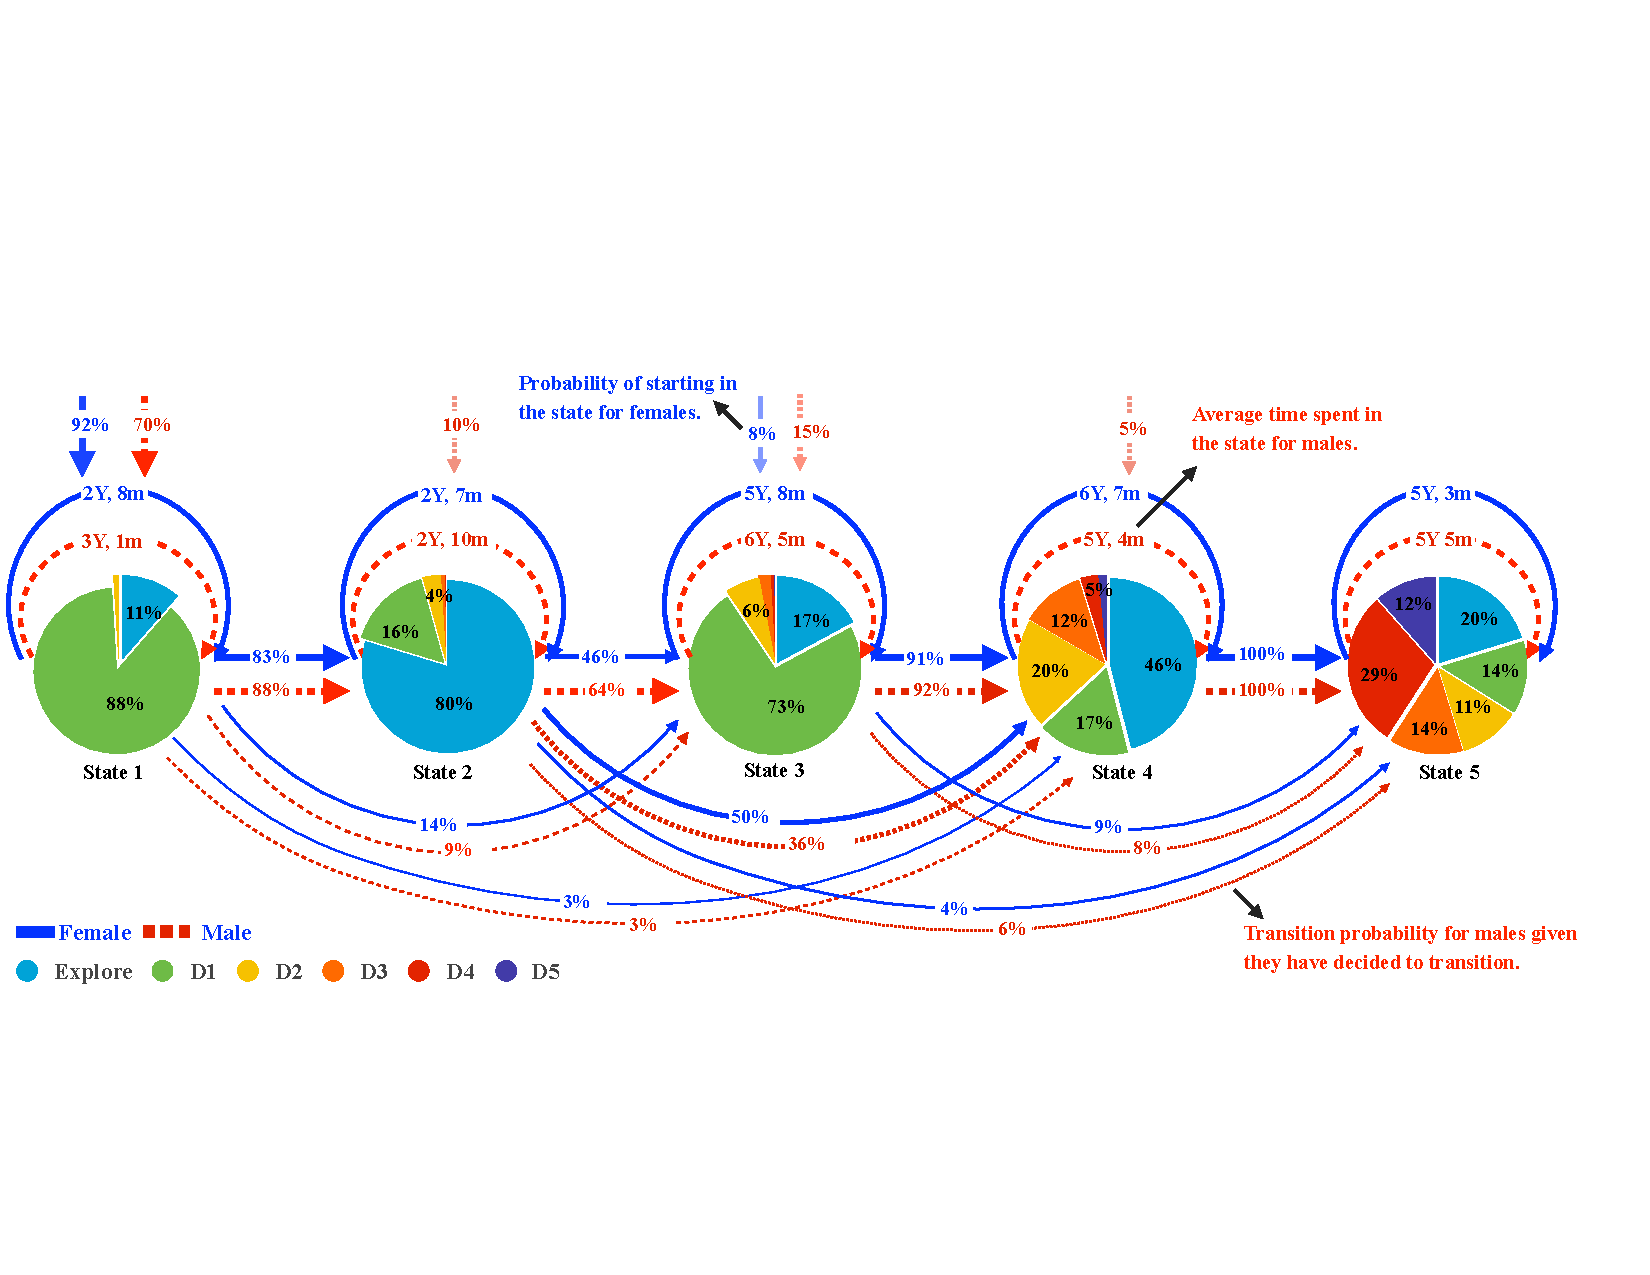
\includegraphics[width=1\linewidth,height=7cm]{figures/Cluster3_both_Self.pdf}
    \caption{
    \label{fig:genderacadclusters} Gender wise representation of trajectory for researchers belonging to the \emph{diverse} archetype in the Academic Dataset. The transitions in blue denote transition probabilities of female professors in the archetype while those in red represents probabilities for their male counterparts. Men start their career from later evolved stages while women make long term state transitions.}
    \label{fig:academic_gender}
\end{figure*}

For the sake of brevity, we examine gender difference in only the \emph{diverse} archetype in some detail. ~\Cref{fig:academic_gender} shows three interesting variations. First, we observe that women are much more likely to start in state 1 (92\%), with a dominant area of interest ($D_1$) than in any other state. In contrast, men start in states 1, 2, 3, and 4, with only 70\% starting in state 1. Both men and women skip stages, but women are more likely to skip a stage than men. For example, 50\% of women skip stage 3, while only 36\% of men do. Longer skips of two stages are rarer, and both women and men make these long skips at the same rate. Finally, there are clear differences between mid-career men and women (states 3, 4): women spend more time \emph{exploring} mid-career (state 4) than men, and mid-career men spend more time in their starting area of interest ($D_1$, state 3) than women.

\subsection{Grant income variability across Archetypes \& gender within an Archetype}
\label{sec:grant}
We next examine the relationship between variation in the academic trajectories and gender to research grants awarded at different stages of an academic career. We extract historical information of grants from the National Science Foundation, a large federal funding agency for Science \& Engineering in the United States \footnote{\url{bit.ly/nsfgrants}}. We consider grants with Principal Investigators (PI) from the same subset of CS professors in top-50 US universities as in~\Cref{sec:discussion}. We collect information for 1062 professors and manually disambiguate names and identify gender by cross-validating with the researcher's webpage.
Then, we compute the average grant money awarded to a researcher, at each stage in their trajectory. ~\Cref{fig:grantanalysis}, which shows letter-value plots of average grant size awarded as PI's, broken down by archetypes (steady, diverse, evolving or diffuse), stage within an archetype and gender, summarizes our findings.

\begin{figure*}[tbh]
    \centering
    \begin{subfigure}{0.5\linewidth}
        \centering
        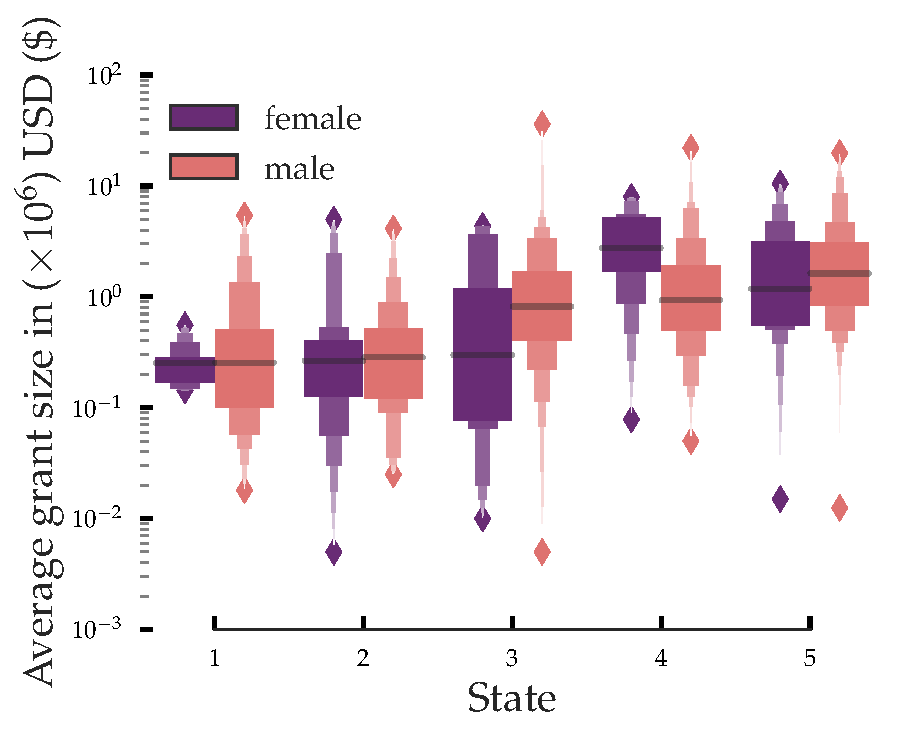
\includegraphics[width=0.8\linewidth,height=5cm]{figures/Cluster_4_PI_grant.pdf}
        \caption{Steady Researchers}
    \end{subfigure}%
    \begin{subfigure}{0.5\linewidth}
        \centering
        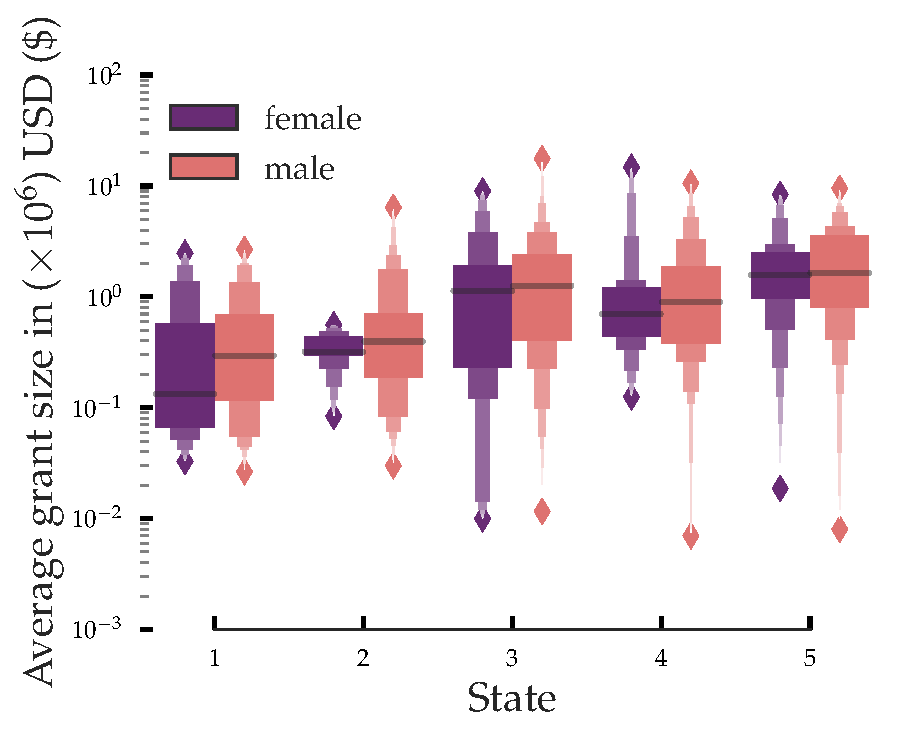
\includegraphics[width=0.8\linewidth,height=5cm]{figures/Cluster_3_PI_grant.pdf}
        \caption{Diverse Researchers}
    \end{subfigure}
    \begin{subfigure}{0.5\textwidth}
        \centering
        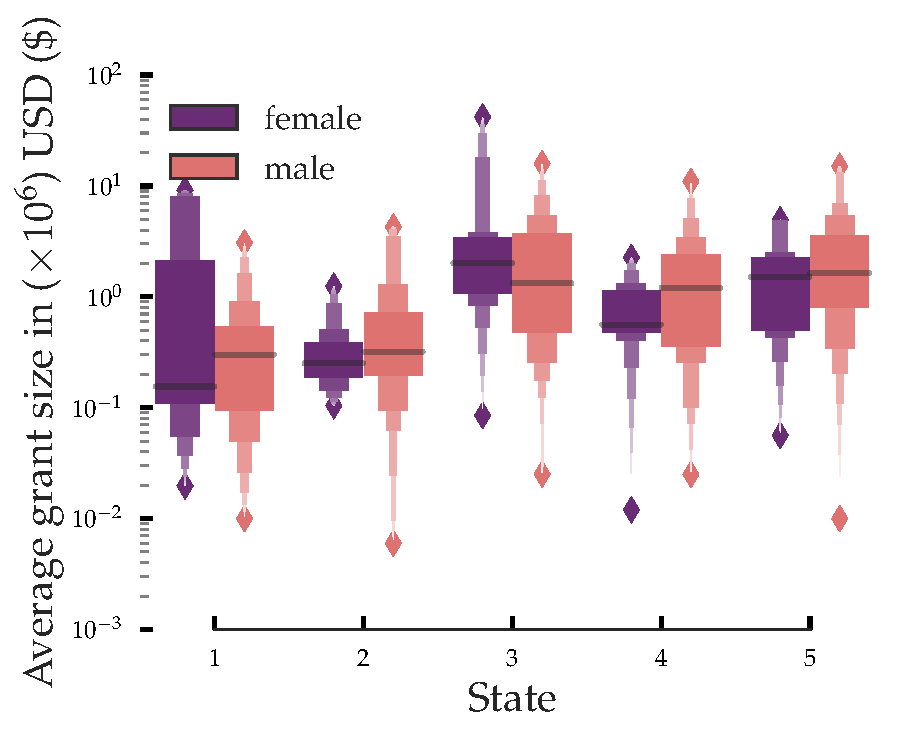
\includegraphics[width=0.8\linewidth,height=5cm]{figures/Cluster_1_PI_grant.pdf}
        \caption{Evolving Researchers}
    \end{subfigure}%
    \begin{subfigure}{0.5\textwidth}
        \centering
        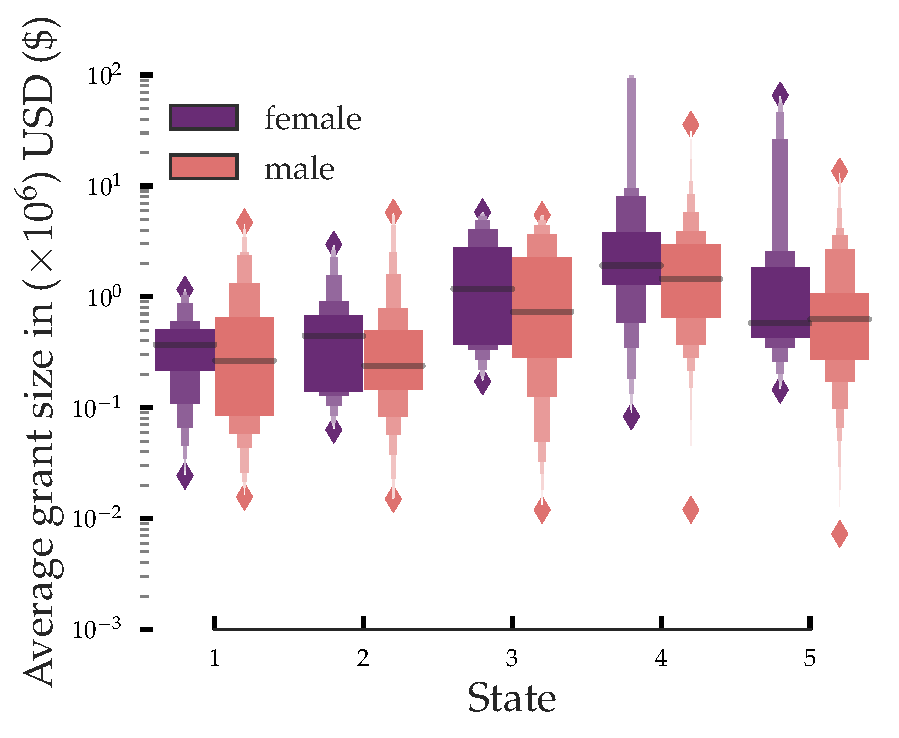
\includegraphics[width=0.8\linewidth,height=5cm]{figures/Cluster_2_PI_grant.pdf}
        \caption{Diffusive Researchers}
    \end{subfigure}
    \caption{\small \label{fig:grantanalysis} Letter value plots of total grant money awarded by NSF when author is a PI in each stage. In general, Professors get more grant money as they gain experience. Regardless of archetypes, grant income in state 3 is significantly higher from state 2 (p< .01). There are also significant differences across genders within a state of an archetype. For instance, for Evolving archetype, male professors get significantly more income than female professors in state 4 (p < .01).}
\end{figure*}

\begin{table}[tbh]
\centering
\begin{tabular}{ll}
\toprule
Archetype (H-test) &  State Pair (t-test)  \\
\midrule
\multirow{2}{*}{Steady***}    & State 2 vs 3**    \\
                     & State 4 vs 5*    \\
\hline
\multirow{2}{*}{Diverse***}   & State 2 vs 3*** \\
                                    & State 4 vs 5*    \\ \hline
\multirow{3}{*}{Evolving***}  & State 2 vs 3***   \\
                         & State 3 vs 4*    \\
                        & State 4 vs 5**    \\ \hline
\multirow{1}{*}{Diffuse***}   & State 2 vs 3***     \\
\bottomrule
\end{tabular}
\caption{ \small Statistical significance tests for the differences in grant money across latent states within an archetype. Shown are only those tests that are statistically significant. H-test \cite{Kruskal:1952} confirms that at least one state is different from another state of the archetype; t-test \cite{Welch:1947} was then conducted between each consecutive states within the archetype to determine the differing states. $* = p < .1, ** = p< .01, *{*}* = p < .001$ }
\label{tab:statstate}
\end{table}


Additionally, we conducted Kruskal-Wallis H-test~\cite{Kruskal:1952} to establish the statistical significance of differences in grant money across latent states within an archetype. This test affirms that at least one latent state is different from another latent state within an archetype \footnote{ We also conducted H-test for the difference in average grant income across archetypes for the same state. However, we did not find any significant differences. \Cref{fig:grantanalysis} can easily verify this lack of difference. }. We then conducted Welch's t-test~\cite{Welch:1947} between consecutive states to find the exact pair of states which are significantly different. We only tested with consecutive latent states as we are only interested in grant income changes as the author progresses through stages. ~\Cref{tab:statstate} reports the state pairs for each archetype that are statistically different. In the rest of this section, we describe these results in detail.

Regardless of archetypes, we observe that in general authors tend to receive more grant money as they gain experience in~\Cref{fig:grantanalysis}. On average, across archetypes and gender, PI's receive in state 5, four times the amount of grant money than state 1 ($p < .001$). Also for researchers across archetypes and across genders, we notice an uptick in grant income in state 3 from state 2 ($p < .01$ - ~\Cref{tab:statstate}). Let us qualitatively examine the \emph{steady} researchers in detail, by comparing~\Cref{fig:grantanalysis} with~\Cref{fig:acadclusters}. State 2 in~\Cref{fig:acadclusters} shows the researchers exploring different topics, whereas, in state 3, they are spending a significant part of their time on their main domain $D_1$. Also, notice that 36\% of the researchers never visit state 2 - 27\% skip state 2, and 9\% of the researchers start in state 3. Since state 1 typically represents the time spent by the researchers in their Ph.D., and with 74\% time spent in an explore stage in state 2, it is not surprising that we see limited grant income in their first two states. State 3, perhaps reflects a sustained focus on their domain $D_1$, and this pays off in terms of grant income. Similar qualitative arguments follow for the other archetypes.


\begin{table}%[tbh]
\centering
\begin{tabular}{ll}
\toprule
Archetype & Latent State (t-test) \\
\midrule
\multirow{2}{*}{Steady}   & State 1* \\
& State 4*  \\ \hline
Diverse   &  State 2*  \\ \hline
\multirow{2}{*}{Evolving}  & State 4** \\
& State 5*    \\  \hline
Diffuse & {Not significant}  \\
\bottomrule %\hline
\end{tabular}
\caption{ \small
\label{tab:statgender}Statistical significance tests \cite{Welch:1947} for the differences in grant money across gender in each state within an archetype. Shown are only those tests that are statistically significant. \\ $* = p < .1, ** = p< .05, *{*}* = p < .001$}
\end{table}

However, the grant trajectories over states is different for each archetype ($p < .001$). Let us examine statistically different state pairs from ~\Cref{tab:statstate} in ~\Cref{fig:grantanalysis}. Steady researchers see a big uptick in their grant income in state 3 ($p < .01$) and a dip in state 5 ($p < .1$), perhaps due to switching back to their primary research area. The grant income for diverse researchers (who have more than one dominant area) increases steadily over states($p < .05$). For evolving researchers (who change their dominant area), the grant income rises (state 3, $p < .001$), falls (state 4, $p < .05$) and rises (state 5, $p < .1$), reflecting a degree of unpredictability accompanying \emph{changing area of interest}. Diffuse researchers see an increase in funding in state 3 ($p < .001$) with similar grant income in subsequent states.

To determine differences in grant income across gender, we further conducted t-test \cite{Welch:1947} between grant distributions of female and male professors in each state within an archetype. ~\Cref{tab:statgender} reports significantly different states within each archetype. We again examine these statistically different states from ~\Cref{tab:statgender} in ~\Cref{fig:grantanalysis}. Evolving women receive significantly \emph{lower} income than evolving men when they \emph{switch to new areas} in state 4 and 5 ($p < .05$). On the other hand, in our dataset, steady women receive significantly \emph{higher} grant income than steady men when they \emph{switch areas} in state 4 ($p < .05$). In general, we observe that men show greater grant income variability than do women. The variability is statistically significant ($p < .05$) during early career in state 1 and 2 for Steady and Diverse researchers respectively. We do not observe significant differences in grant income of male and female Diffusive researchers.


\subsection{StackOverflow Archetypes}
\label{sec:stack}
\begin{table}[!h]
	\centering
	\begin{tabular}{p{30mm} p{25mm} p{25mm} p{25mm} p{25mm}@{}}
		\toprule
		  & Experts & Seekers & Enthusiasts & Facilitators \\
		\midrule
		State 1& \{14.4S\} \newline $\mathbf{A}$ (68\%) \newline C (19\%) &
		\{3.7S\} \newline $\mathbf{Q}$ (69\%)\newline C (19\%)&
		\{12.6S\} \newline $\mathbf{C}$ (42\%)\newline \textbf{Q} (39\%) &
		\{15.4S\} \newline $\mathbf{Q}$(50\%) \newline C (32\%) \\
		State 2 &  \{17.8S\} \newline \textbf{C} (60\%)\newline ${A}$ (25\%) &
		\{8.4S\} \newline \textbf{C} (51\%)\newline ${Q}$ (33\%) &
		\{9.5S\} \newline \textbf{A} (49\%)\newline ${C}$ (32\%) \newline ${E}$ (12\%)&
		\{26.4S\} \newline \textbf{C} (44\%) \newline ${A}$ (28\%) \newline ${E}$ (22\%)\\
		State 3 & \{9S\} \newline $\mathbf{A}$ (87\%)  &
		\{2.2S\} \newline $\mathbf{A}$ (84\%) &
		\{3.7S\} \newline $\mathbf{E}$ (82\%) &
		\{8.4S\} \newline $\mathbf{A}$ (87\%)  \\
		State 4 & \{12.3S\} \newline $\mathbf{C}$ (82\%)  &
		\{5.3S\} \newline $\mathbf{C}$ (72\%) \newline ${Q}$ (15\%) &
		\{9S\} \newline $\mathbf{C}$ (75\%) \newline $A$ (10\%)  &
		\{24.2S\} \newline $\mathbf{C}$ (68\%) \newline $\mathbf{A}$ (14\%) \newline $E$ (13\%) \\
		State 5 & \{5S\} \newline $\mathbf{E}$ (45\%) \newline {C} (28\%) \newline ${A}$ (21\%) &
		\{3.7S\} \newline $\mathbf{Q}$ (85\%) &
		\{10.5S\} \newline $\mathbf{Q}$ (40\%) \newline {C} (33\%) \newline ${E}$ (16\%) &
		\{14.3S\} \newline \textbf{E} (63\%) \newline ${C}$ (22\%) \\
		State 6 & \{11S\} \newline $\mathbf{C}$ (48\%) \newline {A} (38\%)  &
		\{7.7S\} \newline $\mathbf{C}$ (55\%) \newline \textbf{Q} (23\%) \newline ${E}$ (11\%) &
		\{5S\} \newline $\mathbf{A}$ (61\%) \newline {C} (23\%) \newline ${E}$ (11\%) &
		\{21S\} \newline \textbf{C} (57\%) \newline ${E}$ (24\%) \newline ${A}$ (13\%) \\
		\bottomrule
	\end{tabular}
	\caption{\label{tab:stackexchangemean} Learned mean vector for each state for four archetypes in the Stack Overflow Dataset. We list the \emph{activities} in sorted order and annotate them with their \% contribution in the state. We list main activities ($>$ 11\%) for each state. Each state is also labeled with it's average number of sessions. The labels reflect our own interpretation of the user behavior.}
\end{table}

We now describe archetypes learned for the Stack Overflow data. Table \ref{tab:stackexchangemean} depicts the latent states for all archetypes. We label the 4 archetypes discovered as \emph{Expert}, \emph{Seekers}, \emph{Enthusiasts} and \emph{Facilitators}. Posting Comments is the most frequent activity in all archetypes as it is a very low cost activity. Moderator actions and Edits are least favored activities by Stack Overflow users. Most of the users spend initial sessions for \emph{posting questions} (state 1) and significant proportion of their later sessions in \emph{posting answers or comments} (state 6).

\texttt{Experts} users join the community to answer queries or post clarifications or edit answers (state 1-6). They spend at least 68\% of their sessions in \emph{posting answers} (state 1 \& 3). They rarely ask questions of their own. In
communities like Stack Overflow, it is vital to have a dedicated group of experts answering queries for it to be sustainable.

\texttt{Information Seekers}
join the community for getting answer to their queries accounting for 69\% of activities per session (state 1). They briefly start contributing by posting answers to the community (state 3) but they end up again in \emph{commenting} (state 6) or \emph{asking questions} (state 5).

\texttt{Enthusiasts} start by asking questions and posting comments (state 1). They, then, start answering questions and commenting on other answers (state 2). They briefly stay (4 sessions) in edit state (state 3) but end up migrating to either commenting again (state 4) or asking questions and commenting (state 5). We denote them as \emph{Enthusiasts} as they use the platform to post questions while simultaneously answering queries from their acquired knowledge.

\texttt{Facilitators} join for information seeking (state 1) but start posting answers, clarifying and editing in state \emph{2-3}. However, later on they take a more subdued approach and only post comments. The reason for this decreased interest is hard to gauge but identifying these users and retaining their interest could be important to sustain the community.


In summary, we identify four dominant archetypes for researchers: steady, diverse, evolving, and diffuse. We observe differences in the evolution of male and female researchers within the same archetype. When we examine the diverse archetype in detail, we observe that women and men differ in where they start, rate of transition, and time spent in mid-career. The differences in grant income are salient across states within an archetype. In general, grant income increases with experience. We also observe differences across genders within a stage of an archetype mostly accompanied by an area switch. Finally, we also identified dominant archetypes for StackOverflow community: experts, information seekers, enthusiasts and facilitators.
